\documentclass[a4paper, 12pt]{article}
\usepackage[T1]{fontenc}
\usepackage{lmodern}
\usepackage{color}
\usepackage{amsfonts}
\usepackage{epstopdf}
\usepackage{matlab}
\usepackage{booktabs}
%\documentclass{book}
\usepackage{blindtext}
\usepackage{hyperref}
\usepackage[brazil]{babel}
\usepackage{amssymb}
\usepackage[utf8]{inputenc}
\usepackage{amsmath}
\usepackage{indentfirst}
\usepackage{graphicx}
\usepackage{listings}
\usepackage{tcolorbox}
\usepackage{upgreek}
\usepackage{multicol,lipsum}
\usepackage[a4paper,
top=3cm, left=3cm, bottom=3cm, right=3cm]{geometry}
\usepackage{setspace}
\usepackage{multirow}
\usepackage{float}
\usepackage[dvipsnames]{xcolor}
\usepackage[table]{xcolor}
%\usepackage{pdflscape}
\usepackage[DIV=15]{typearea}
\usepackage[nottoc]{tocbibind}
\usepackage[sort,numbers]{natbib}
%\usepackage{cite}
\usepackage{matlab}

\usepackage[utf8]{inputenc}
\usepackage[T1]{fontenc}
\usepackage{lmodern}
\usepackage{graphicx}
\usepackage{color}
\usepackage{hyperref}
\usepackage{amsmath}
\usepackage{amsfonts}
\usepackage{epstopdf}
\usepackage[table]{xcolor}
\usepackage{matlab}


\documentclass[letterpaper]{article}
% bib pack %%%%%%%%%%%%%%%%%%%%%%%%%%%%%%%%%%%%%%%%%%%%%%%%%%%%%%%%%%%%%%%%%%%%%
\usepackage[utf8]{inputenc}
\usepackage{geometry}
    \geometry{left=3cm,right=2cm,top=2cm,bottom=2cm}
%
\usepackage[spanish]{babel}
%
\usepackage[fixlanguage]{babelbib}
    \bibliographystyle{babunsrt}
%
\usepackage{url}

\begin{document}
%\maketitle

\begin{titlepage}
	\begin{center}
		

\vspace{10pt}
%\begin{figure}[H][!ht]
%\centering
%
\includegraphics{puc-rio-logo.png}

%\end{figure}
\begin{figure}[!ht]
\centering

\includegraphics{images/puc-rio-logo.png}
\end{figure}
\huge{Instrumentação Eletrônica}
        \vspace{70pt}
        
		\textbf{ENG1027}
		\textbf{\large{\\ }}
		
		\vspace{30pt}
		\textbf{\small{\\ Circuitos de Pontes}}
		\vspace{75pt}
		
	\end{center}
	
	\begin{flushleft}
		\begin{tabbing}
			Alunos\qquad\qquad\=\>Paloma Sette - 1621595\\
			\>Renan Sued - 1621618 \\
			Professor\>Igor Braga de Paula\\
	\end{tabbing}
		  
	\end{flushleft}
	\begin{center}
		%\vspace{\fill}
		\vspace{215pt}
		Rio de Janeiro, 11 de Junho de 2023
	\end{center}
\end{titlepage}
%%%%%%%%%%%%%%%%%%%%%%%%%%%%%%%%%%%%%%%%%%%%%%%%%%%%%%%%%%%
\newpage
\tableofcontents
\thispagestyle{empty}

\newpage
\pagenumbering{arabic}

\newpage

%\newcommand{\listequationsname}{Lista de Equações}
%\newlistof{myequations}{equ}{\listequationsname}
%\newcommand{\myequations}[1]{%
%\addcontentsline{equ}{myequations}{\protect\numberline{\theequation}#1}\par}

%\listofmyequations
\newpage


\newpage

\listoffigures
\thispagestyle{empty}

\newpage
%%%%%%%%%%%%%%%%%%%%%%%%%%%%%%%%%%%%%%%%%%%%%%%%%%%%%%%%%
%%%%%%%%%%%%%%%%%%%%%%%%%%%%%%%%%%%%%%%%%%%%%%%%%%%

\newpage

\thispagestyle{empty}

\newpage

\section*{Introdução}
Este relatório refere-se à prática experimental de circuitos de pontes, da disciplina de Instrumentação Eletrônica (ENG1027) de 2023.1. 
Para as simulações, utilizaremos o software LTSpice.

\section{Circuito de Pontes}

Foi visto em sala de aula que circuitos com arranjo em ponte são úteis para medição precisa de
resistência, capacitância e indutância. Um arranjo para medição de resistências, conhecido como ponte
de WheatStone é ilustrado abaixo:
 \\
\begin{figure}[H]
\centering
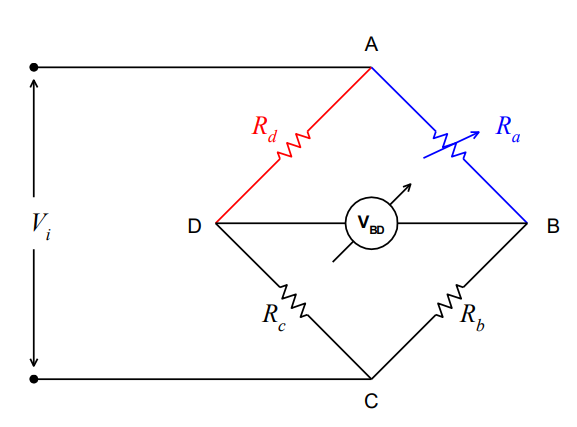
\includegraphics[scale = 0.65]{images/ponte.png}
\label{filtro1}
\caption{Ponte de WheatStone}
\end{figure}

Deseja-se montar um circuito para medição da variação de resistência de extensômetros (\textit{strain gauges})
que possuem resistência nominal de $120 \Omega$. A alimentação da ponte será feita com uma fonte de $5V$,
a corrente máxima que pode passar pelo sensor é de $50mA$.\\

No experimento, foram escolhidos os componentes e foi feita a montagem da ponte. Foi colocado o strain gauge a ser medido no lugar do componente com impedância $R_d$ (conforme desenho).

\newpage
\subsection{Primeiro passo}
Nesta etapa, foi necessário escolher os componentes para a montagem da ponte sem que a corrente máxima fosse ultrapassada.\\

Componentes para montagem da ponte:

\begin{itemize}
    \item \textbf{Resistores fixos $R_a$, $R_b$, $R_c$ e $R_d$: }Podem ser escolhido com um valor próximo à resistência nominal do extensômetro, ou seja, próximo a 120 Ohms.
    \item \textbf{Extensômetro (\textit{strain gauge})}: Substituir o componente com impedância $R_d$ pelo extensômetro de 120 Ohms.
\end{itemize}\\

Portanto, resumidamente, podemos definir

\begin{equation*}
    R_a = R_b = R_c = R_d = 120 \Omega
\end{equation*}

Dessa forma, a corrente será dividida igualmente entre os ramos da ponte e não ultrapassará a corrente máxima de 50mA.


\begin{itemize}
    \item \textbf{Extensômetro (\textit{strain gauge})}: 1k$\Omega$.
\end{itemize}





\newpage
\subsection{Segundo passo}
 Com base na escolha feita. Estimar qual vai ser a relação entre $R_a$ e $R_d$.\\

A relação entre $R_a$ e $R_d$ determina a sensibilidade da ponte de Wheatstone. Para encontrar a relação, precisamos considerar o equilíbrio da ponte, onde a tensão nos pontos médios dos resistores é zero. Nesse caso, a relação é dada por:\\


\begin{equation*}
\frac{R_a}{R_d} = \frac{R_b}{R_c}
\end{equation*}\\

Para os valores escolhidos anteriormente, a relação será de $1 \Omega$ .



%Portanto, a relação entre Ra e Rd é igual à relação entre $R_b$ e $R_c$. Neste caso, como Ra e Rb são escolhidos com valores próximos e $R_c$ é maior, a relação $R_a / R_d$ será próxima de 1.\\

%\begin{equation*}
%    120 * 1000 = 120 * Rd
%\end{equation*}

%\begin{equation*}
%    Rd = 1000 \Omega = 1k\Omega
%\end{equation*}







\newpage
\subsection{Terceiro passo}
 Com $R_a$ constante, estimar qual vai ser a variação de voltagem para uma resistência $R_d$ arbitrária.\\

Para $R_a$ fixo e $\Delta V \neq 0$, temos que a ponte está em desequilíbrio.\\

A variação de voltagem na ponte de Wheatstone é proporcional à variação de resistência. Essa variação é dada pela seguinte equação:

\begin{equation*}
    \frac{\Delta V}{V} = \frac{R_b}{R_a + R_b} - \frac{R_c}{R_c + R_d}
\end{equation*}


Onde:
\begin{itemize}
    \item $\Delta V$ é a variação de voltagem na ponte de Wheatstone.
    \item V é a tensão de alimentação da ponte (5V no  caso).

\end{itemize}

%Portanto, se conhecermos a variação de resistência $\Delta R_d$ de um extensômetro específico, podemos estimar a variação de voltagem $\Delta V$ dividindo $\Delta R_d$ por $R_d$ e multiplicando pelo valor de tensão $V$ da fonte de alimentação da ponte.\\

%Importante ressaltar que, para garantir que a corrente máxima de 50mA não seja ultrapassada, é necessário considerar os valores dos resistores escolhidos e realizar os cálculos de acordo com as leis de Ohm e as condições específicas do circuito.\\

Portanto, a variação de voltagem para uma resistência $R_d$ arbitrária poderá ser, considerando uma variação de resistência  $ R_d = 200 \Omega $.\\ \\


\begin{equation*}
\Delta V = 5(\frac{120}{120 + 120} - \frac{120}{120 + 200}) = 0,625 V
\end{equation*}

Portanto, para um valor de resistência de 200 $\Omega$ em $R_d$, por exemplo, teríamos uma variação de voltagem de $625 mV$ na saída da ponte.




\newpage
\subsection{Quarto passo}
Comparar cálculos teóricos com simulações, para os dois modos de operação:

\begin{itemize}
    \item Detecção de nulo. Demonstrar sensibilidade.
    \item Por deflexão. Demonstrar sensibilidade do circuito.
\end{itemize}

\subsubsection{Por detecção de nulo}
Neste caso, teremos a ponte balanceada ($\Delta V = 0$), i.e.:

\begin{equation*}
    R_a R_c = R_b R_d \>\ \longrightarrow \>\ R_d = \frac{R_a R_c}{R_b}
\end{equation*}

\begin{figure}[H]
\centering
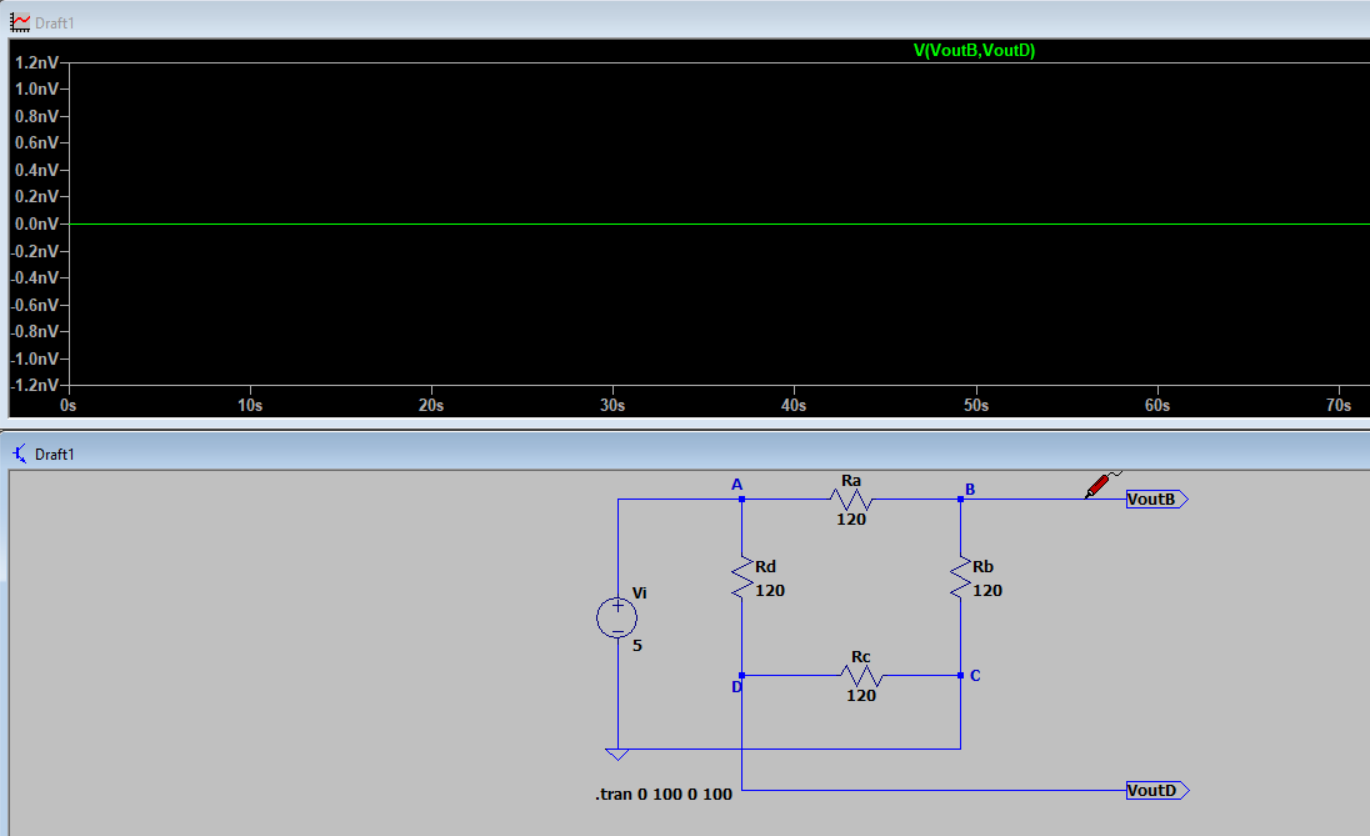
\includegraphics[scale = 0.45]{images/4.1.png}
\caption{Ponte de WheatStone - LTSpice - Detecção de nulo - q.04}
\end{figure}


\subsubsection{Por deflexão}
Neste caso, temos a ponte desbalanceada ($\Delta V \neq 0$), i.e.:

\begin{equation*}
    \frac{\Delta V}{V} = \frac{R_b}{R_a + R_b} - \frac{R_c}{R_c + R_d}
\end{equation*}

\begin{figure}[H]
\centering
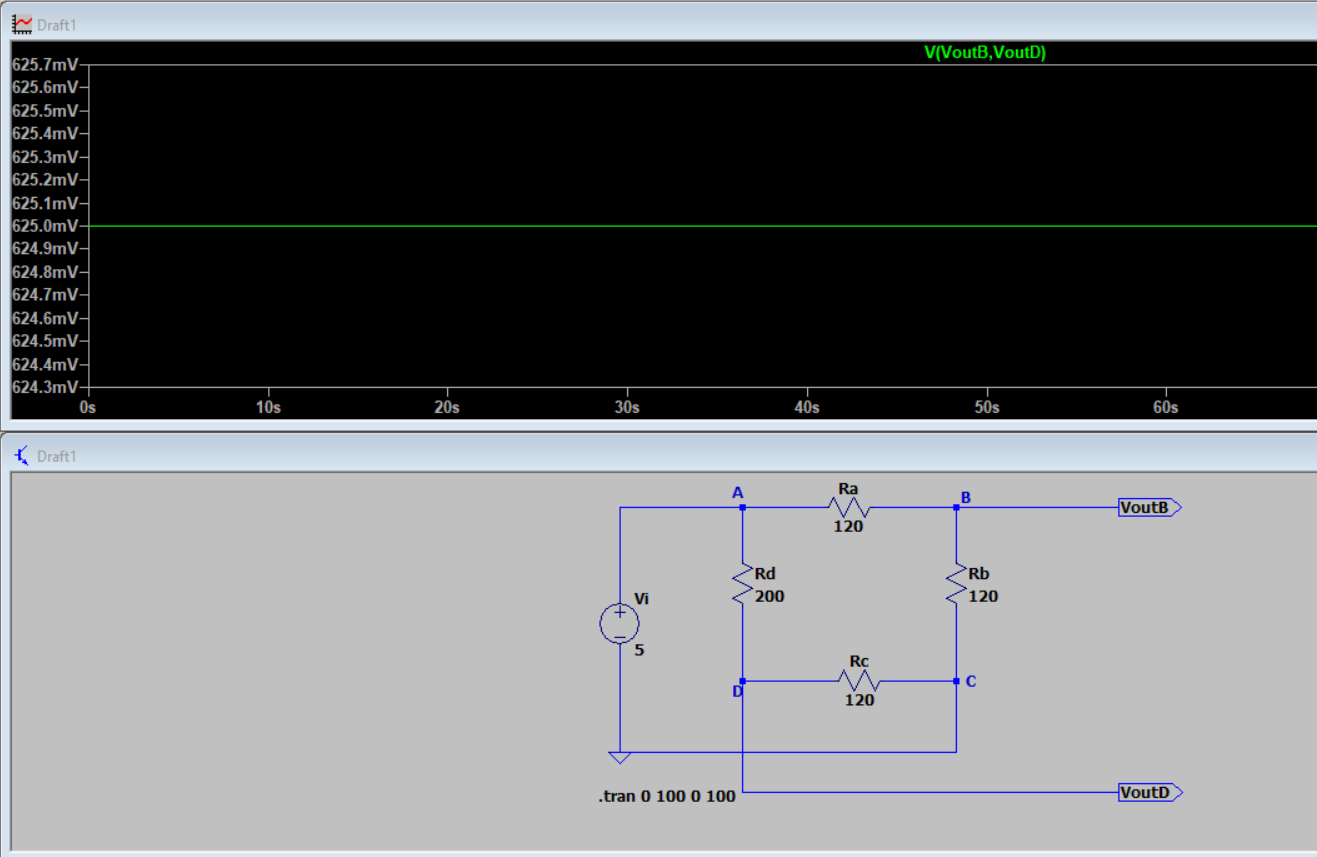
\includegraphics[scale = 0.45]{images/4.2.png}
\caption{Ponte de WheatStone - LTSpice - Deflexão - q.04}
\end{figure} \\ 

Portanto, concluímos que a simulação está fazendo sentido, pois arbitramos a resistência $R_d$ de acordo com o exemplo da questão anterior e obtivemos exatamente o valor de $525 mV$.

%\newpage
%\subsection{Quinto passo}
%Na simulação, substitua o Strain Gauge por um Termistor e simule a variação de temperatura na faixa entre 10$^{\circ}$C e 60$^{\circ}$C. Verificar a resposta do circuito.\\






%\newpage
%\subsection{Sexto passo}
%Faça uma montagem de ponte de WheatStone para medição de capacitâncias, conforme slides do
%curso. Defina uma conjunto capacitor com resistência interna a ser medido (chutar valores, lembrando
%que as resistências internas são tipicamente baixas). Mostre como é feita a medição iterativa com esse
%circuito (variar resistências e mostrar como VBD diminui até que se atinge um ponto a partir do qual
%qualquer variação das resistências ajustáveis causa um aumento na tensão VBD).\\


\newpage
% REFERENCIAS %%%%%%%%%%%%%%%%%%%%%%%%%%%%%%%%%%%%%%%%%%%%%%%%%%%%%%%%%%%%%%


\end{document}